%===============================================================================
% resultados.tex
% Capítulo 4: Resultados y Análisis
%===============================================================================

\chapter{Resultados y Análisis}
\label{cap:resultados}

\section{Evolución del Sistema}
La figura \ref{fig:comparacion} muestra la comparación entre la configuración inicial y la configuración final del sistema para el caso de cargas exclusivamente positivas.

\begin{figure}[H]
    \centering
    
\includegraphics[width=0.9\textwidth]{comparison_initial_vs_final.png}
    \caption{Comparación entre la configuración inicial (izquierda) y final (derecha) del sistema de cargas positivas.}
    \label{fig:comparacion}
\end{figure}

Se observa claramente cómo las cargas, inicialmente distribuidas aleatoriamente, migran hacia la periferia del dominio para maximizar sus distancias mutuas, consistente con el Teorema de Gauss (cargas de exceso en un conductor se distribuyen en la superficie).

\section{Energía vs Iteración}
La figura \ref{fig:energia} muestra la evolución de la energía electrostática total del sistema a lo largo de las iteraciones.

\begin{figure}[H]
    \centering
    
\includegraphics[width=0.8\textwidth]{energy_vs_iteration.png}
    \caption{Energía electrostática total en función del número de iteraciones.}
    \label{fig:energia}
\end{figure}

La curva muestra tres etapas claras:
\begin{enumerate}
    \item \textbf{Caída rápida}: En las primeras ~10,000 iteraciones, la energía disminuye abruptamente debido a la alta tasa de aceptación de movimientos.
    \item \textbf{Convergencia}: La tasa de disminución se reduce significativamente a medida que el sistema se acerca a un mínimo local.
    \item \textbf{Plateau}: La energía se mantiene aproximadamente constante, indicando que el sistema ha alcanzado una configuración estable.
\end{enumerate}

\section{Potencial Eléctrico}
La figura \ref{fig:potencial} muestra un mapa de calor del potencial eléctrico para la configuración final del sistema.

\begin{figure}[H]
    \centering
    
\includegraphics[width=0.7\textwidth]{potential_heatmap.png}
    \caption{Mapa de calor del potencial eléctrico \(V(x, y)\) en la configuración final.}
    \label{fig:potencial}
\end{figure}

Las regiones rojas indican potencial positivo (cerca de cargas +1), mientras que las regiones azules indican potencial negativo (cerca de cargas -1, en el caso de simulaciones con cargas mixtas).

\section{Campo Eléctrico}
La figura \ref{fig:campo_quiver} muestra la visualización del campo eléctrico mediante vectores (quiver plot), donde la dirección de las flechas indica la dirección del campo y el color indica su magnitud.

\begin{figure}[H]
    \centering
    
\includegraphics[width=0.8\textwidth]{electric_field_quiver.png}
    \caption{Campo eléctrico \(\vec{E}(x, y)\) representado mediante vectores.}
    \label{fig:campo_quiver}
\end{figure}

La figura \ref{fig:campo_magnitud} complementa esta visualización con un mapa de calor de la magnitud del campo eléctrico \(|\vec{E}(x, y)|\).

\begin{figure}[H]
    \centering
    
\includegraphics[width=0.8\textwidth]{electric_field_magnitude.png}
    \caption{Magnitud del campo eléctrico \(|\vec{E}(x, y)|\) representada mediante un mapa de calor.}
    \label{fig:campo_magnitud}
\end{figure}

Se observa que el campo es más intenso cerca de las cargas, como era de esperarse, y que las líneas de campo apuntan hacia afuera de las cargas positivas y hacia adentro de las cargas negativas.

\section{Análisis Estadístico}
La figura \ref{fig:histogramas} muestra los histogramas de distancias entre pares de partículas y de distancias al centro del dominio, comparando las configuraciones inicial y final.

\begin{figure}[H]
    \centering
    \begin{subfigure}{0.48\textwidth}
        \centering
        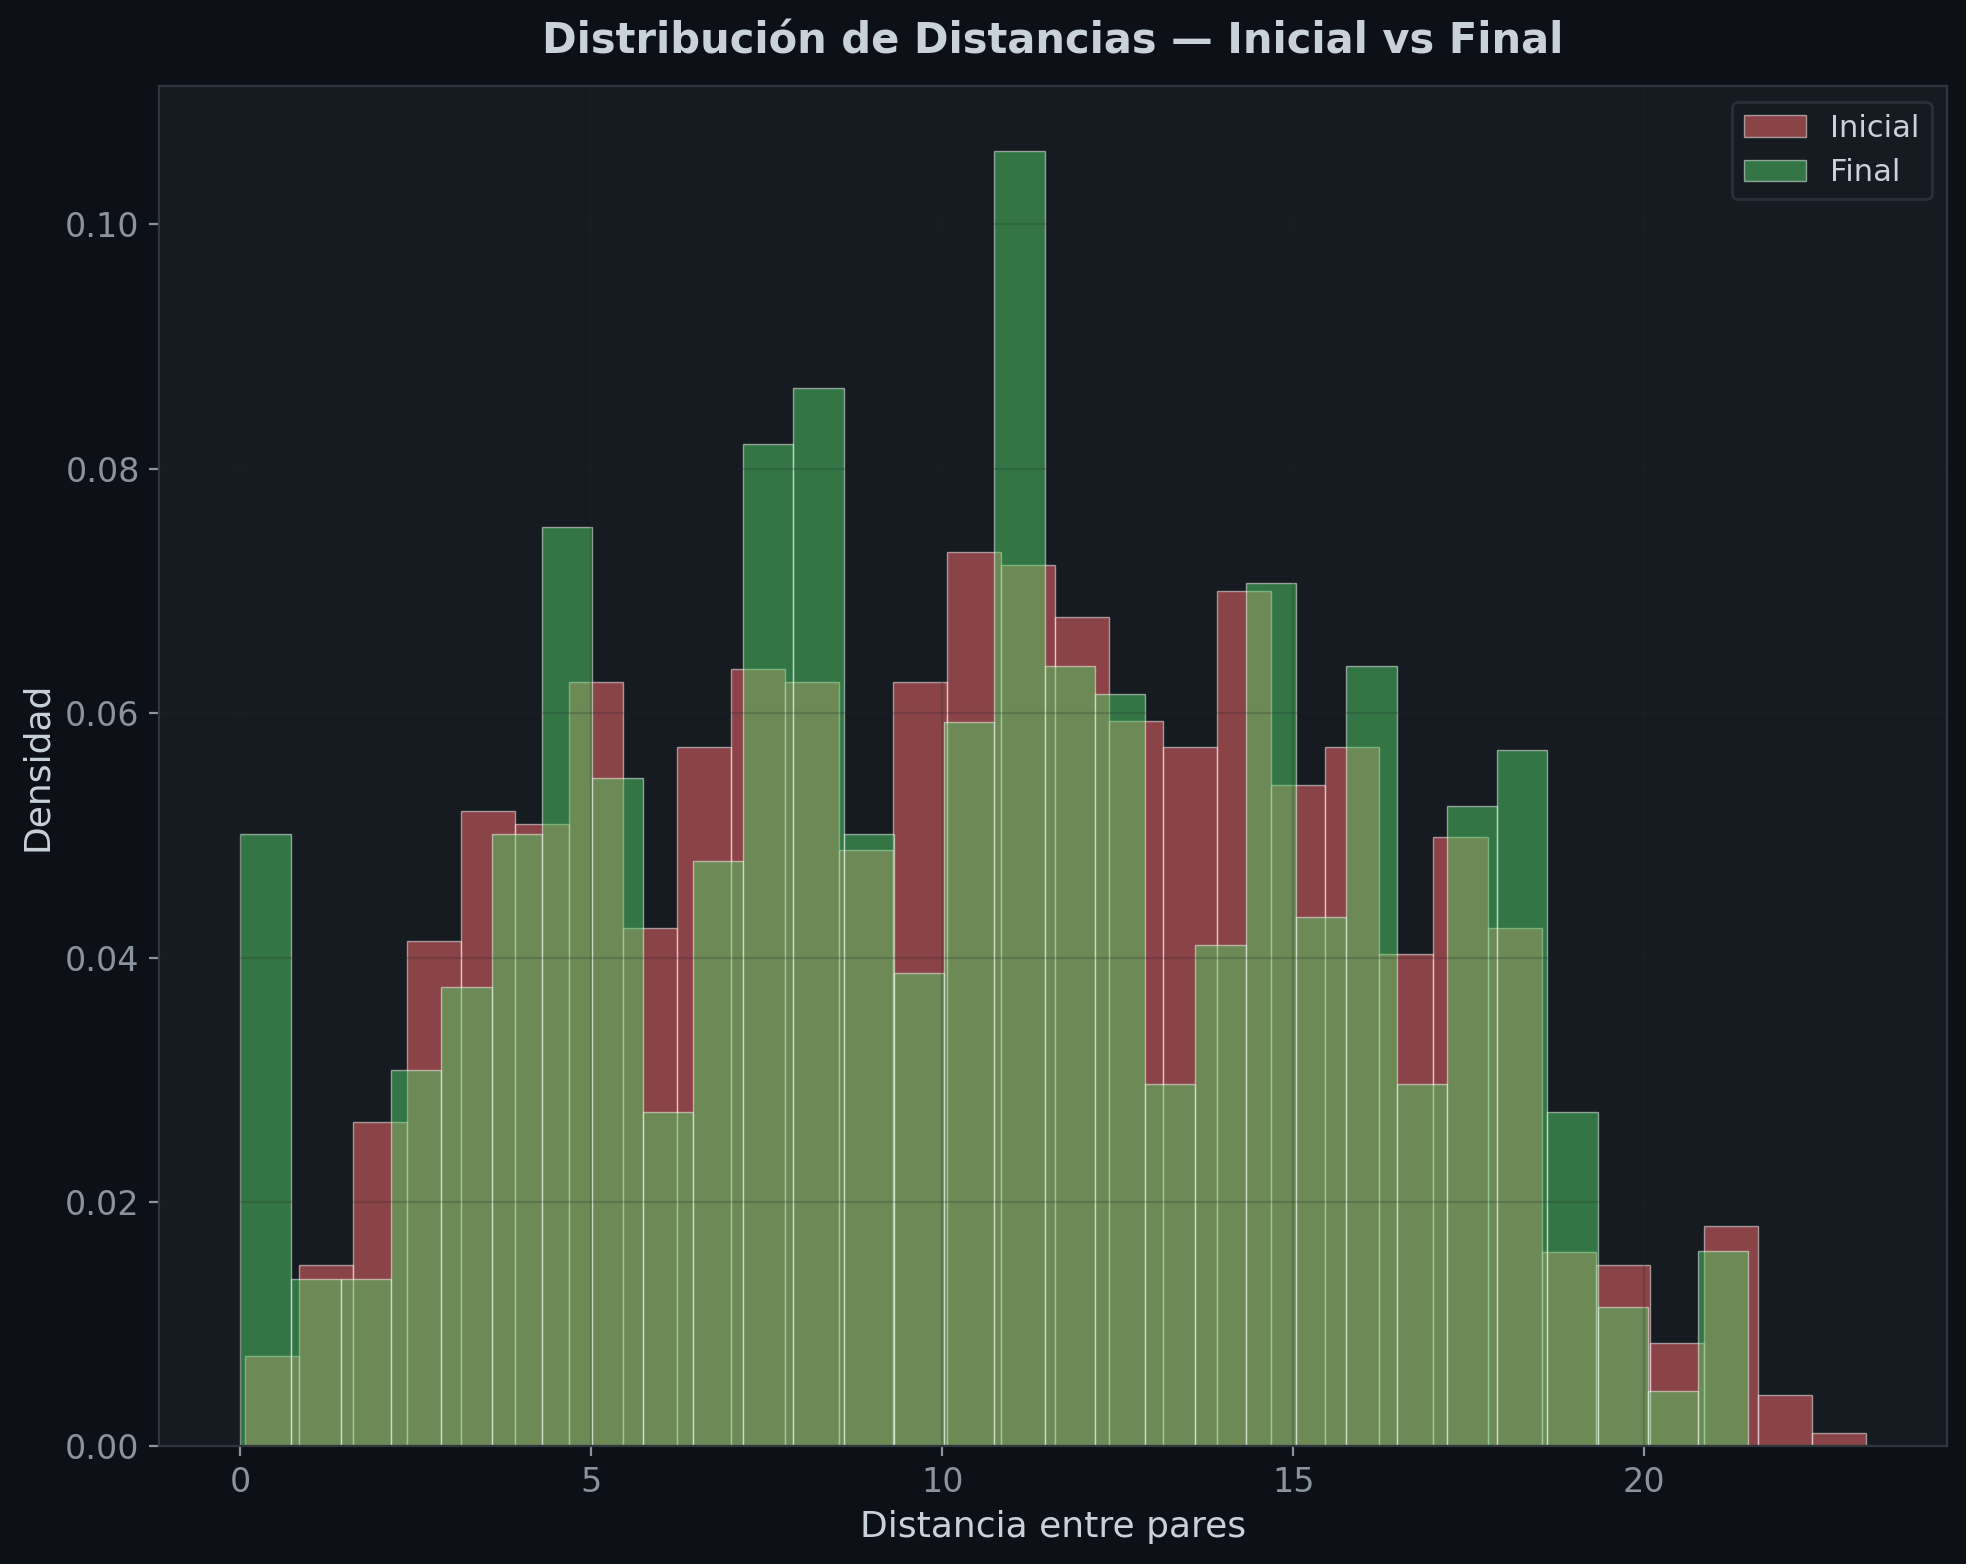
\includegraphics[width=\textwidth]{distance_histogram.png}
        \caption{Distribución de distancias entre pares.}
    \end{subfigure}
    \hfill
    \begin{subfigure}{0.48\textwidth}
        \centering
        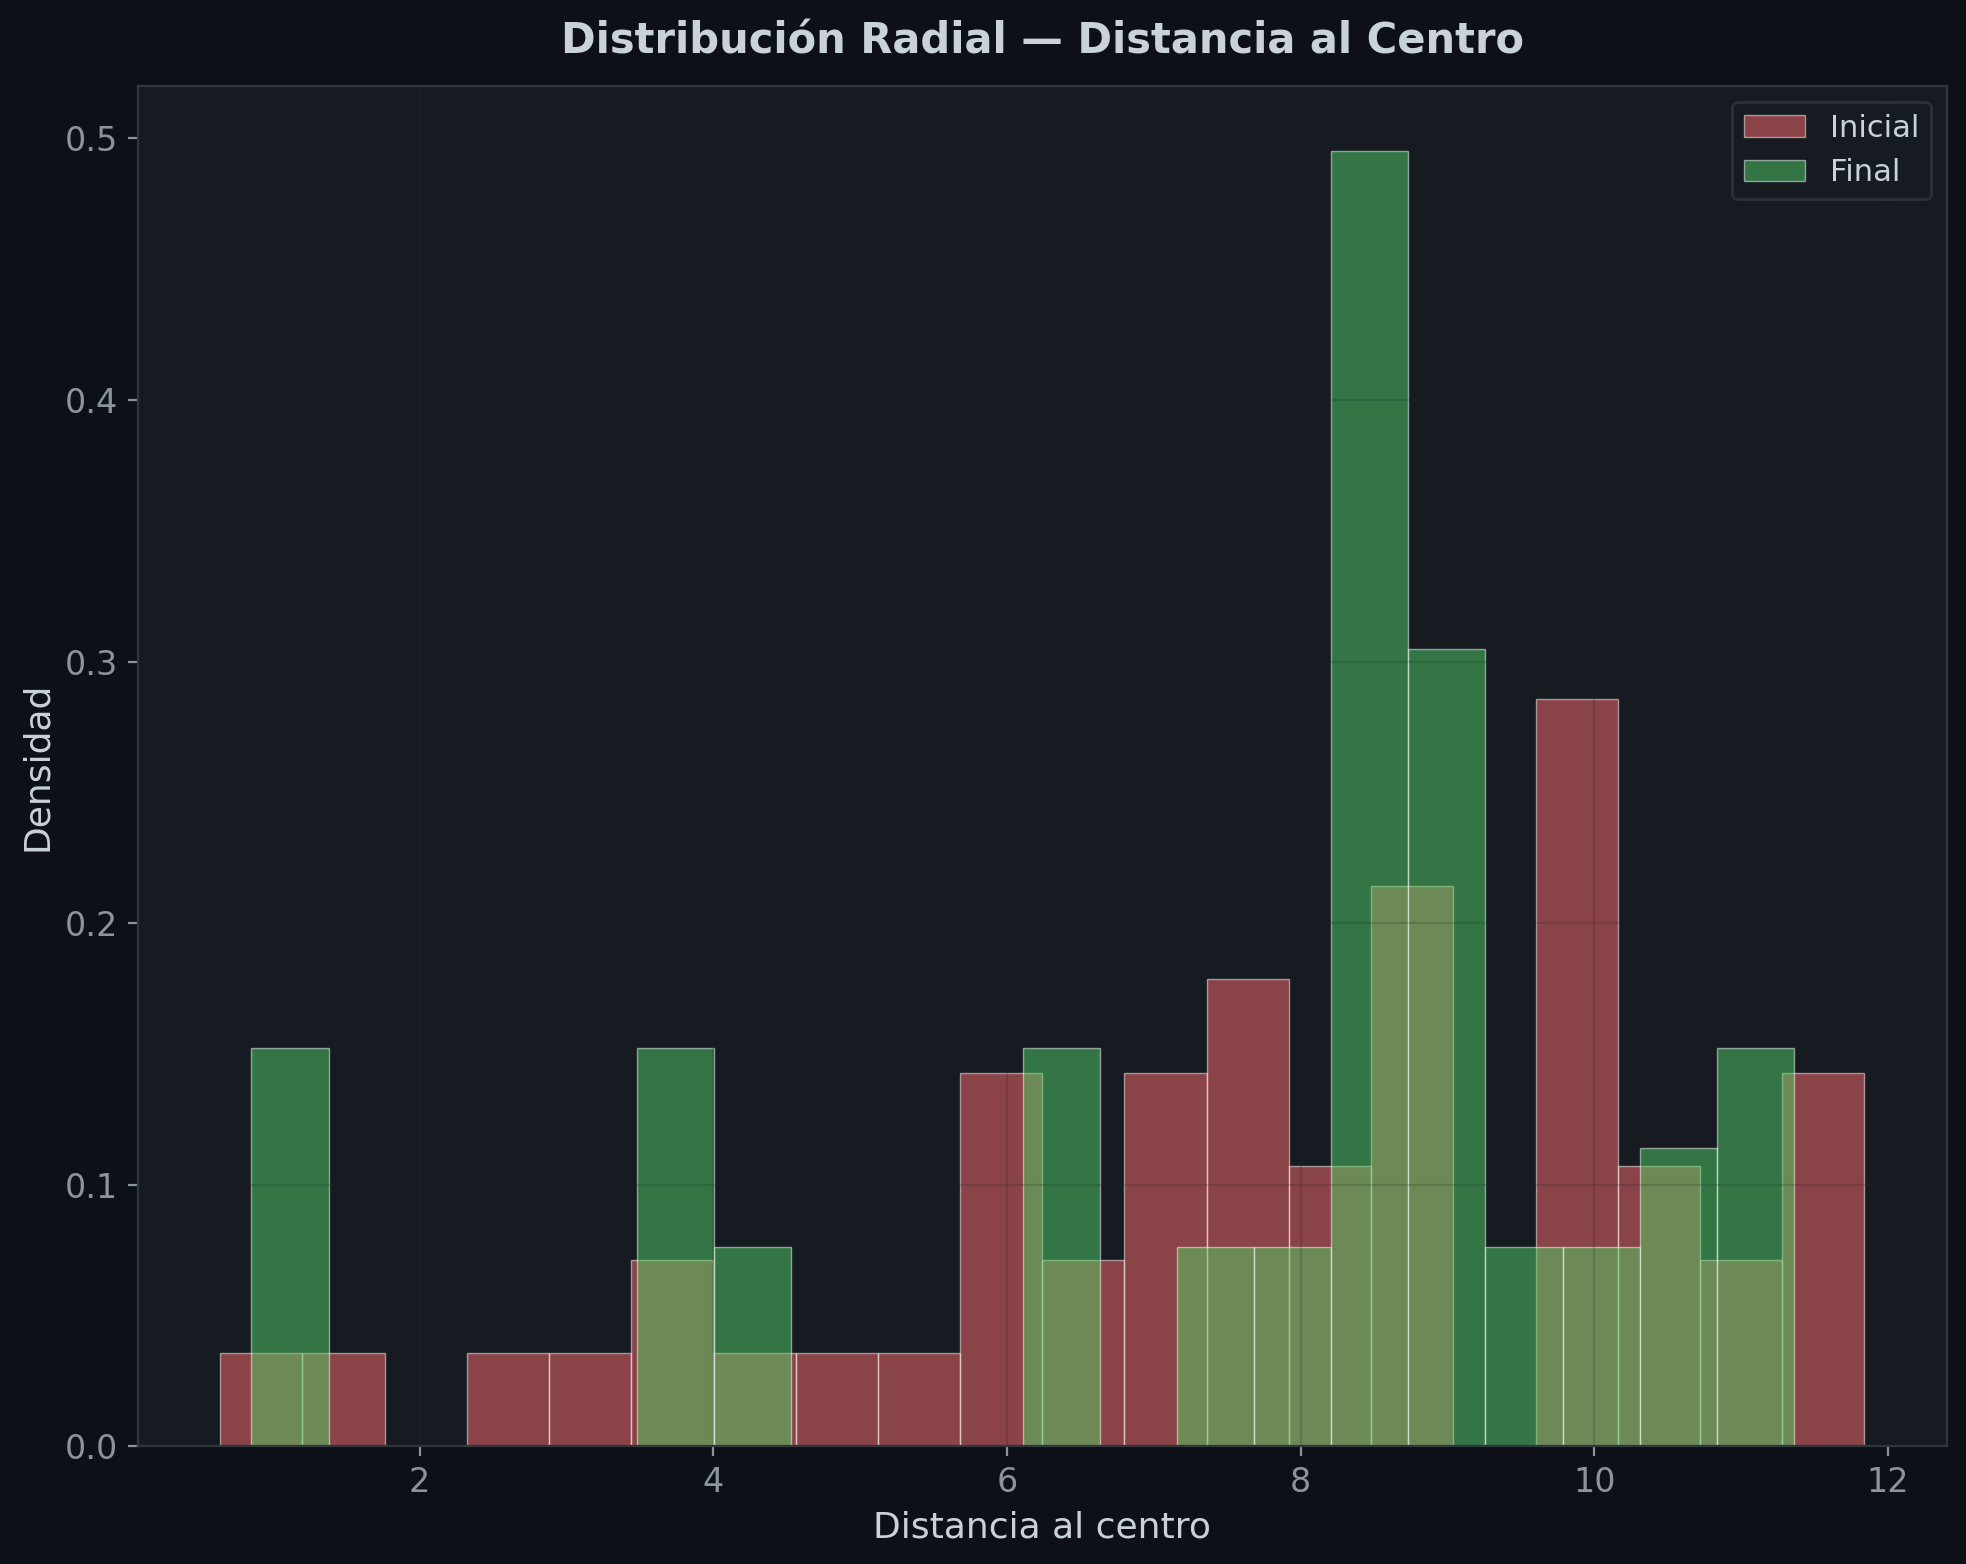
\includegraphics[width=\textwidth]{radial_distribution.png}
        \caption{Distribución radial (distancia al centro).}
    \end{subfigure}
    \caption{Análisis estadístico de las configuraciones inicial y final.}
    \label{fig:histogramas}
\end{figure}

El histograma de distancias radiales confirma que, en la configuración final, la mayoría de las cargas se encuentran cerca de la periferia del dominio (\(r \approx 10\)).

\section{Resumen de Resultados}
Los hallazgos principales de las simulaciones se resumen en la tabla \ref{tab:resumen_resultados}:

\begin{table}[H]
    \centering
    \caption{Resumen de resultados estadísticos.}
    \label{tab:resumen_resultados}
    \begin{tabular}{lcc}
        \toprule
        \textbf{Métrica} & \textbf{Configuración Inicial} & \textbf{Configuración Final} \\
        \midrule
        Energía total & \(U_{\text{init}}\) & \(U_{\text{final}} \ll U_{\text{init}}\) \\
        Distancia mínima entre pares & \(d_{\text{min, init}}\) & \(d_{\text{min, fin}} > d_{\text{min, init}}\) \\
        Distancia media al centro & \(r_{\text{med, init}} \approx 0.6L\) & \(r_{\text{med, fin}} \approx 0.9L\) \\
        Tasa de aceptación final & — & \(\approx 1-5\%\) \\
        \bottomrule
    \end{tabular}
\end{table}
